\section{Background}\label{background}
\subsection{Background}

\subsubsection{Determinants of populist voting}

[IP: this subsection is redundant with what comes before - I think that the lit survey on the determinants of populist voting is what's already in the introduction. I don't think we need to repeat it here] 

Populism thrives on the interaction between long-term economic transformations and cultural backlash. Key economic drivers include trade globalization, automation, and deindustrialization, which have left many regions—particularly rural and peri-urban areas—economically vulnerable. In parallel, cultural and identity-based grievances, often reinforced by status anxiety and perceived marginalization, further catalyze populist support.

In the US and Europe, the collapse of industrial employment, rising inequality, and falling social mobility have been shown to predict populist voting patterns (\cite{Autor2020}; \cite{Dippel2015}; \cite{Colantone2018}). In France, for example, \cite{Malgouyres} and  \cite{Algan2017} document that regions more exposed to import competition or economic negative shocks are also those where far-right support has increased most markedly.

Cultural backlash is another key driver of populist voting. \cite{Inglehart2016} argue that the rise of populism reflects a reaction against the erosion of traditional cultural values, particularly among older, less-educated, and more socially conservative voters who feel threatened by rapid cultural change, immigration, multiculturalism, and gender equality. \cite{Gidron2017} further highlight the role of status anxiety, showing that individuals with declining subjective social status are significantly more likely to support populist parties. \cite{Algan2017} show that distrust in political institutions and interpersonal trust are strong predictors of populist support, while \cite{Giuliano2020} and \cite{Rodriguez2021} find that declining social capital in peripheral areas correlates with higher populist vote shares. 

The 2008–09 global financial crisis and subsequent austerity programs were catalyzers of the populist sentiment. Fiscal austerity in the UK boosted support for right-wing populist parties (\cite{Fetzer2019}; \cite{Vries}). While much of the literature has focused on the negative political consequences of state withdrawal, relatively few studies provide causal evidence on the effects of positive redistribution. The aforementioned papers are among the rare exceptions (\cite{ALBANESE2022}; \cite{Becker2017}).


\subsubsection{Front National (FN)}

The FN was established in 1972, emerging from the remnants of various extreme-right groups (some Waffen-SS, members of the OAS, neo-Nazis and Vichy's nostalgic).\footnote{Organisation de l'Armée Secrète, a terrorist group that fought to keep Algeria as French.} Jean-Marie Le Pen played a pivotal role in uniting various factions under a common nationalist and populist agenda. The party's rhetoric and provocative statements, particularly Le Pen's controversial remarks about the Holocaust, garnered substantial media attention and public debate. 

The National Front's electoral breakthrough began in the March 1982 cantonal elections, where candidates reached or exceeded 10\% of the vote in places like Grande-Synthe (13.3\%) and Dreux-Est (19.6\%). Its rise is often traced to the March 1983 municipal elections, notably when Jean-Marie Le Pen received 11.26\% in Paris and a coalition in Dreux earned 31\% in the first round. The National Front gained national prominence in the June 1984 European elections, securing 10.95\% of the vote and ten seats in the European Parliament, marking its "entry into politics." On March 16, 1986, with a new proportional voting system, the National Front won 35 seats in the National Assembly.

Initially, the FN promoted economic liberalism and anti-communism, reflecting the right-wing and nationalist sentiments of its founders.\footnote{Published in 1978, "Doctrine économique et sociale du Front National", by Pierre Gérard, "a kind of 'liberal-national' manifesto that 'revisits Poujadist ideas and praises economic freedoms,' according to \cite{igounet2014}, would serve as the party's reference on economic issues until 1990."} However, as globalization and economic changes affected its voter base, the FN shifted towards a more protectionist and welfare-oriented economic stance. P.-A. Taguieff described this transition as a move from "national-liberalism" to "national-populism".\footnote{Pierre-André Taguieff, sociologist and historian, is the director of research at the French National Centre for Scientific Research (CNRS) in an Institut d'études politiques de Paris laboratory, the Centre for Political Research (CEVIPOF)} It was marked by advocating for policies that protect French jobs and industries from foreign competition, criticizing the European Union's economic policies, and promoting social welfare programs framed as benefiting "native" French citizens over immigrants. Specifically after the fall of the Berlin Wall, the National Front underwent a shift that led it, in the words of Bruno Mégret, to choose the camp of "nationalism" over "globalism." In his 2002 presidential platform, Jean-Marie Le Pen declared, "It is imperative to regulate trade with a measured protectionism." Denouncing "ultra-free-trade," the National Front leader aimed to "restore economic borders to France (and, if possible, to Europe)."\footnote{The campaign slogan "1  million de chômeurs, c'est 1 million d'immigrés en trop" (A million unemployed is a million immigrants too many) summarizes the FN's "national populism".} Jean-Marie Le Pen added, "We are against the euro, which eliminates France's sovereignty in the economic domain." He added that France must regain "control of its currency and, therefore, control over its economic and financial policy." Eventually, the 2002 presidential election was a turning point for the FN. Jean-Marie Le Pen's surprise qualification for the second round of the election shocked France. He received 16.86\% of the vote, surpassing the Socialist candidate Lionel Jospin. Despite losing to Chirac in the runoff, this event marked the FN's arrival as a significant force in French politics. Marine Le Pen took over the leadership from her father in 2011. Under her leadership, the FN sought to soften its image, distancing itself from the overtly xenophobic and anti-Semitic rhetoric of the past. The re-branding included a name change to "Rassemblement National" (National Rally) in 2018.

Initially, the FN resonated with a poujadist electorate composed mainly of small urban traders and artisans, employed and generally educated.\footnote{"Poujadism", named after Pierre Poujade, was a far-right political and trade union movement in France that emerged in 1953 in the Lot and dissolved in 1958. It advocated for the protection of small business owners and artisans, who were seen as threatened by the post-war expansion of large retail chains, and criticized the inefficacy of parliamentary governance under the Fourth Republic. The movement, associated with the Union de défense des commerçants et artisans and its political arm, Union et fraternité française, used strong-arm tactics in demonstrations and engaged in combative protests. Often seen as a "small-bourgeois conservatism," the term "poujadism" has come to refer pejoratively to reactionary, corporatist political movements. Notably, Jean-Marie Le Pen, later the founder of the National Front, began his political career as a Poujadist deputy.} Over time, however, this base shifted, and the FN increasingly attracted those who felt "left behind."

The FN was widely considered a populist party during our period of interest (1995-2002). This classification stems from its rhetoric that pits "the people" against "the elites," its anti-establishment stance, and its appeal to nationalism and sovereignty.\footnote{The American Heritage Dictionary defines populism as "a political philosophy supporting the rights and power of the people in their struggle against the privileged elite."} The party consistently portrays itself as the defender of ordinary French citizens against corrupt elites, both within France and in the broader European context. Its populist approach is characterized by a strong emphasis on national identity, opposition to immigration, and a critique of globalization. 



Figure \ref{fig:fn_vote_share} shows the evolution of the FN vote share in the first rounds of the different presidential elections. The scores of Jean-Marie Le Pen are stable around 13\%, while they reach 23\% in 2022 with Marine Le Pen. Lately, the party rose to prominence during the 2024 European elections by winning the highest vote share among all French political parties, as well as in the 2022 and 2024 legislative elections, and the first rounds of the 2017 and 2022 presidential elections. 


% FN results presidential across time
\begin{figure}[h]
    \centering
    \caption{Evolution of FN Vote Share (1988-2022) - Presidential Elections in France}
    \label{fig:fn_vote_share}
    
    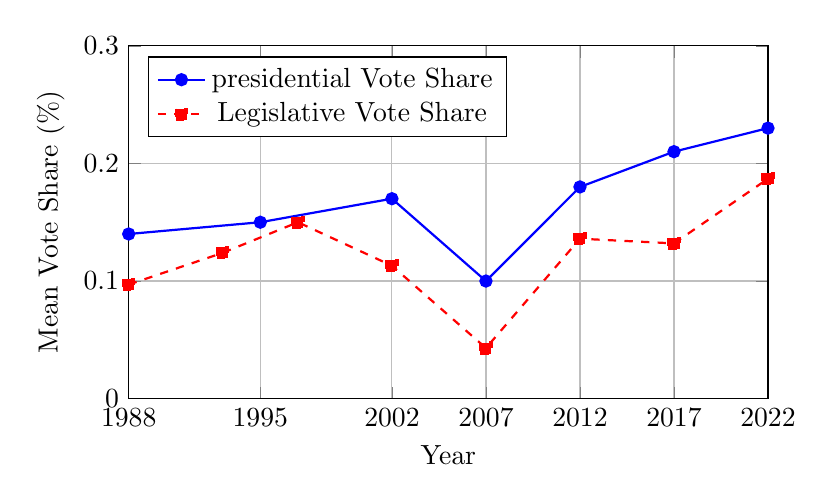
\begin{tikzpicture}
        \begin{axis}[
            width=0.8\textwidth,
            height=0.5\textwidth,
            xlabel={Year},
            ylabel={Mean Vote Share (\%)},
            ymin=0.0, ymax=0.3,
            xmin=1988, xmax=2022,
            xtick={1988, 1995, 2002, 2007, 2012, 2017, 2022},
            ytick={0.0, 0.1, 0.2, 0.3},
            grid=major,
            legend pos=north west,
            xlabel near ticks,
            ylabel near ticks,
            tick label style={/pgf/number format/1000 sep=}
        ]

        % Mean vote share
        \addplot[blue, mark=*, thick] table {
            1988 0.14
            1995 0.15
            2002 0.17
            2007 0.10
            2012 0.18
            2017 0.21
            2022 0.23
        };
        \addlegendentry{presidential Vote Share}
        
         % legislative
        \addplot[red, mark=square*, thick, dashed] table {
            1988 0.097
            1993 0.124
            1997 0.150
            2002 0.113
            2007 0.043
            2012 0.136
            2017 0.132
            2022 0.187
        };
        \addlegendentry{Legislative Vote Share}
        
        
        \end{axis}
    \end{tikzpicture}


\parbox{\textwidth}{\footnotesize \textit{Notes:} The vote shares correspond to the ratio of the number of votes Le Pen (Jean-Marie and, after 2011, Marine Le Pen) received to the total number of expressed votes in the first round of the presidential election.}
    

\end{figure}

\subsubsection{Socioeconomic evolution in rural France}

Non-urban communities are those that lagged behind economically and experienced slower growth in France over the past 30 years. They also are the ones where the electoral support for the FN increased the most in the same period. The literature identifies three main reasons to that differential increase: (i.) composition effect; (ii.) economic and social isolation; (iii.) state withdrawal.\footnote{There are additional and not necessarily contradictory explanations. The influential demographer Hervé Le Bras, in an interview to \textit{Le Monde} in 2022, explains the predominance of rural populist vote with the education-occupation gap: "One of the consequences of the remarkable increase in education levels and the number of graduates [...] is that the level of education individuals achieve no longer corresponds to the positions they occupy in society." In France, while 36\% of the working population have completed higher education, only 16\% are executives and professionals. This mismatch is more pronounced in rural areas: in municipalities with fewer than 1,000 inhabitants, 20\% of baccalaureate holders are white-collar workers, compared to 45\% in cities with more than 100,000 inhabitants."}

\begin{enumerate}
    \item \textbf{Composition effect}

This argument highlights the socio-demographic and economic changes France has experienced since the 1980s. Younger and more educated individuals have migrated to urban areas in search of better opportunities, leaving behind an older and less mobile population. \cite{Guilly2014} notes that the "forced" migration of the "native French" (those with both parents born in France) working class from urban to rural and deep suburban areas, mainly due to rising real estate prices, has created a divide.\footnote{The publication in 2014 of \textit{La France périphérique : Comment on a sacrifié les classes populaires} launched an intense debate in France. The concept "peripheral France" was criticized for its simplicity, but remains relevant in the French public discourse.} This divide separates them from recent immigrant suburbs on one side and the "globalized and gentrified" metropolitan areas on the other. This separation has fostered distrust towards both immigrants and globalized elites, leading to a cultural withdrawal into more socially and culturally homogeneous "hinterlands." Figure \ref{fig:FN_typology} displays the mean vote share for the Front National (FN) across three aggregated typologies—Rural, Intermediary, and Urban—calculated for the years 1988, 1995, 2002, and 2007. The FN vote increased relatively more in rural and intermediary municipalities than in urban ones. Similarly, support for the FN was initially strong among the top-income voters, but has since diminished, whereas support from lower-income deciles has increased. \footnote{\cite{Piketty}, Graph 12.19. While the top-income voters (top 5\% and top 1\%) intially showed strong alignment with the "droite nationale," this trend diminished in later years, with growing support emerging from lower-income deciles. The graph is available at the following link: https://www.unehistoireduconflitpolitique.fr/livre.html (chapter 12)} 


% Figure \ref{fig:bartik1990-1999} shows the evolution of the Bartik values I constructed. I explain the construction of the Bartik indicator in Appendix \ref{app:bartik}. I make three main observations:  the Paris region experienced the highest growth between 1990 and 1999; the metropolitan areas look like bright "islands" of growth; "diagonal of emptiness", from the South-West to the North-East of France, is the area that suffered the most in France, along with the non-urban municipalities. It approximately corresponds to the area that the ZRR tried to capture.


\begin{figure}
    \centering
    \caption{Mean FN Vote Share by Urbanization Category}
    \includegraphics[width=1\linewidth]{figures/FN_typologie.png}
    \label{fig:FN_typology}

\parbox{\textwidth}{\footnotesize \textit{Notes:} The figure displays the mean vote share for the Front National (FN) across three aggregated typologies—Rural, Intermediary, and Urban—calculated for the years 1988, 1995, 2002, and 2007. The typologies were regrouped as follows: the "Rural" category includes "rural autonome peu dense," "rural autonome très peu dense," "rural sous faible influence d'un pôle," and "rural sous forte influence d'un pôle"; the "Intermediary" category corresponds to "urbain densité intermédiaire"; and the "Urban" category corresponds to "urbain dense." Each bar represents the average FN vote share for a given typology and year, with values displayed inside the bars. This figure illustrates temporal and spatial variations in FN support across different levels of urbanization.}
    
\end{figure}

% \begin{figure}
%    \centering
%    \caption{Bartik value change between 1990 and 1999}
%    \includegraphics[width=1\linewidth]{figures/bartik_1999_1990_light.png}
%    \label{fig:bartik1990-1999}
%
%\parbox{\textwidth}{\footnotesize \textit{Notes:} The map shows the evolution of the Bartik values between 1990 and 1999 by municipality. A positive Bartik value corresponds to a positive economic shock, while a negative value corresponds to a negative economic shock.}
%    
% \end{figure}

    \item \textbf{Economic and social isolation}

Many non-urban areas have faced economic decline due to deindustrialization, loss of local businesses, and reduced investment. \cite{Guilly2014} notes that this segment of society, characterized by redundancy schemes ("plans sociaux") and deindustrialization, political abstention, or support for the Front National (FN), is forming a sort of "counter-society" that engages in social and cultural re-rooting. "Place" has become the base of local identity, mirroring the findings of \cite{Arzheimer_Bernemann_2024} in Germany. Cultural shifts (multiculturalism, gender equality, and other progressive values) have contributed to a perceived decline in relative status among traditional working-class communities. \cite{Gidron2017} observe a strong association between status anxiety and the populist vote in the US. Additionally, demographic changes in already low-density areas may be accompanied by declining social capital, similar to what happened in the US (\cite{putnam2000}). Evidence suggests that this decline in the US favored support for Trump (\cite{Giuliano2020}; \cite{Rodriguez2021}).

In France, \cite{Lebras2022} identifies a historical division between two Middle Ages landscapes: the bocage regions in the West and Southwest, characterized by scattered farms and hamlets, and the open-field regions in the Northeast and Mediterranean, where populations concentrate in towns and villages. By the late 20\textsuperscript{th} century, the Northeast faced an industrial decline, while the West experienced industrial growth, particularly in the food sector. Social mobility stagnated in the East after the "thirty glorious years" (J. Fourastié, 1979), leading to deteriorating conditions, social disconnection, and a rise in FN support. Meanwhile, improved connectivity and mobility in the West fostered optimism. This analysis motivated me to include the density of fences (haie) per square kilometer [YS: how hard would it be to change it to sq km per agricultural land? IP: not straightforward at all, feasible but costly]as a measure of bocage areas.\footnote{I used satellite data from the Institut national de l'information géographique et forestière (National Institute of Geographic and Forest Information). See the Data section \ref{data-section} for more information.} 


    \item \textbf{State withdrawal}

Non-urban communities often lack essential public services like healthcare, education, postal services, and public transportation. Hospitals, schools, and other critical services have been closed or consolidated, forcing residents to travel farther for basic needs. \cite{davoine2019} shows that this decrease in public infrastructure in rural areas boosts electoral support for populist parties. Additionally, government investments in infrastructure, such as roads, public transportation, and broadband internet, have often favored urban and metropolitan areas.

France's tradition of administrative centralization concentrates decision-making and resources in major cities and regions. This reduces the political influence and autonomy of non-urban areas, making it harder for local governments to address their specific needs. Consequently, this exacerbates economic and social isolation and fuels resentment against the state. \cite{boyer2020} shows that the Yellow Vest movement, initially a grassroots protest against the increase of a tax on gasoline, stands out by having numerous decentralized gathering points, often around roundabouts, far away from Paris.



\end{enumerate}

\subsubsection{The ZRR Program}

The rural revitalization zones (ZRR) were established by the Law of February 4, 1995, on spatial planning and territorial development. The law sought to "correct inequalities in living conditions among citizens" and ensure balanced territorial development. It recognized the necessity of implementing strengthened "positive discrimination" policies for areas facing specific difficulties due to demographic decline and geographical, economic, or social challenges.


\textit{\textbf{Eligibility to the program}} - The ZRR program, officially launched in September 1996, specifically targeted rural employment. Eligibility was determined using a complex algorithm based on demographic, economic, and institutional criteria. To qualify for ZRR status, a county had to have a population density below 31 inhabitants per square kilometer, according to the 1990 Census. Additionally, the population or labor force in the area must have declined between the 1982 and 1990 censuses, or the share of agricultural labor employment must have been at least twice the national average. Furthermore, the municipality had to belong to an existing EU zoning scheme known as the Territoire Rural de Développement Prioritaire (TRDP). However, political influences likely meant that beyond these criteria, other unobserved factors played a role in the selection process (\cite{Gobillon}). For a comprehensive description of the ZRR program, see \cite{BEHAGHEL20151}. 

In 2005, new counties were included in the zoning if they met updated eligibility criteria based on the 1999 census, while no counties were withdrawn even if they no longer met the criteria. Specifically, a county needed to have a population density below 31 inhabitants per square kilometer according to the 1999 census to be added to the ZRR program. Additionally, the requirement that a municipality should belong to an inter-communal establishment (EPCI), a group of municipalities jointly managing local public services, was introduced. This replaced the earlier reference to the TRDP zoning. As a result, both the 1990 and 1999 population densities determined inclusion in the program post-2005.

% map of the ZRR program
\begin{figure}
    \centering
    \caption{Map of the ZRR Program}
    \includegraphics[width=1\linewidth]{figures/map_ZRR.png}
    \label{fig:treatmentMap}

\parbox{\textwidth}{\footnotesize \textit{Notes:} Treatment status is determined at the county (\textit{canton}) level. Counties in black entered the ZRR program during its first phase in 1995; counties in dark gray entered after the 2004 reform; counties in light gray were never treated. Boundaries correspond to administrative divisions and population characteristics as defined by the 1999 census.}

    
\end{figure}

\textit{\textbf{Benefits of the program}} - During the initial phase of implementation (1996-2004), incentives were specifically targeted at two types of businesses: newly established ones and small businesses (with fewer than 50 employees). New businesses were eligible for reductions in corporate and business taxes, while small-but-growing firms received temporary payroll tax exemptions (up to 5 years). A significant change occurred in 2005 when a parliamentary amendment unexpectedly made the scheme more generous, introducing substantial, permanent payroll tax cuts for all employees of "public interest organizations" (associations). This lasted until 2008.

As mentioned by a 2014 parliamentary report, "the regime of tax and social security exemptions forms the core of the benefits provided to the ZRR. It symbolizes the perception of equity that rural areas have within the Republic. During their hearings, your rapporteurs noted the strong commitment of local elected officials' associations to these mechanisms."\footnote{Alain Calmette et Jean-Pierre Vigier, Commission du Développement durable et de l'Aménagement du territoire, « Rapport d'information no 2251 sur les zones de revitalisation rurale (ZRR) », Assemblée nationale, 8 octobre 2014.} In 2013, when nearly 2,000 municipalities were abruptly removed from the classification, the elected officials put enough pressure to have them reinstated a few months later. This episode highlighted the commitment of elected officials to maintaining a system perceived as a symbol of territorial equity policies.\footnote{Another parliamentary report (available at the following link https://www.vie-publique.fr/files/rapport/pdf/104000069.pdf)
 also points out the commitment of rural mayors to the ZRR program (\cite{zrr_evaluation}). }

\textit{\textbf{Size of the program}} - The program covered a significant portion of rural France, amounting to about 39\% of the French territory but only around 8\% of the population. The budgetary cost of the ZRR program before 2005 was approximately of 100 million euros (\cite{Lorenceau2009}), and 400 million euros after 2005. Using the estimates from \cite{BEHAGHEL20151} that compares the French urban EZ program (Zones franches urbaines) with the ZRR, in 2008, payroll tax exemptions amounted to 315 million euros in the urban EZ program (for about 68,000 jobs in 18,000 plants), compared to 200 million euros for Public Interest Organizations (PIOs) in the ZRR program (for about 38,500 jobs in 3,300 plants) and 38 million euros for other firms in the ZRR program (for about 9,000 jobs in 6,000 plants).

\textbf{\textit{Timing of the program}} - The program was voted on in February 1995 but was not launched until September 1996. The 1995 presidential elections took place in April, and the legislation may have already affected the results, particularly if the signaling effect was dominant. As a baseline, I take the 1988 elections to be the last pre-treatment election.\footnote{In section \ref{app:1995signal}, I report results relative to the 1995 elections.}

\textit{\textbf{EZ Literature}} - As described in \cite{Neumark2010}, the Enterprise Zone (EZ) literature encounters significant identification challenges. The designation of EZs is a highly political and endogenous process, often tied to unobserved trends in outcomes, making it difficult to find suitable control groups for these zones. Additionally, program effects may be confounded by other geographically targeted initiatives. 

Furthermore, \cite{KlineMoretti2013} build a spatial equilibrium model where the welfare effects of place-based policies are critically dependent  on the elasticity of housing supply and labor mobility. In areas where housing markets have excess supply, as might be the case in certain rural zones, EZ can improve welfare by raising employment and wages without inflating rents, potentially achieving the program's redistributive goals more effectively.\footnote{Later on, I add the rate of vacant houses per municipality as a control variable.}

In the US, \cite{AustinGlaeserSummers2018} argues that the recent slowdown in regional economic convergence, particularly in areas like the American heartland, underscores the value of geographically targeted policies. Considering the rise of the support for populism in these areas, it feels urgent to consider if EZ can play a role in mitigating it.

In this context, my analysis benefits from a particularly advantageous setting. The designation of rural enterprise zones under the ZRR program followed a centralized process, utilizing preexisting jurisdictions based on 1990 population census data and applying a complex algorithm with a discontinuous population density criterion.


%\textit{\textbf{EZ Literature}} - The literature on Enterprise Zones (EZs) faces significant identification challenges (\cite{Neumark2010}). The designation of EZs is often a politically driven and endogenous process, making it difficult to identify suitable control groups, and program effects may also be confounded by other geographically targeted initiatives. One traditional way to overcome these challenges is to employ a spatial or temporal discontinuity design (RDD or DID), or to use propensity score-matching models. \cite{Billings} analyzes Enterprise Zones in Colorado by using a border-matching methodology that matches EZ and non-EZ areas in close geographical proximity. He finds that EZ fiscal incentives increase the number of employees hired. \cite{MayerEZ} evaluates the "Zones Franches Urbaines" (ZFU) policy in urban areas in France and finds that, conditional on locating in a municipality that hosts a ZFU, the policy has a positive and significant impact on the probability of locating within the ZFU area rather than in the non-ZFU area of the municipality. They estimate the EZ effect using a Difference-in-Differences (DID) methodology and various probability models, comparing areas that belong to the same municipality (within variation). In a theoretical paper, \cite{KlineMoretti2013} presents a spatial equilibrium model suggesting that the effects of EZ policies depend heavily on the elasticity of housing supply and labor mobility. In areas with an excess housing supply, such as certain rural zones, EZs can potentially increase employment and wages without driving up rents.\footnote{To capture this dynamic, I later include the rate of vacant houses per municipality as a control variable.} In the U.S., \cite{AustinGlaeserSummers2018} argue that the recent slowdown in regional economic convergence strengthens the case for geographically targeted policies. With growing support for populist movements in the American heartland, it seems increasingly urgent to assess whether EZs could play a role in the local political landscape. Having this in mind, my analysis benefits from a particularly advantageous setting. The designation of rural enterprise zones under the ZRR program in France was managed centrally, using preexisting jurisdictional boundaries based on 1990 census data and applying a complex algorithm with a discontinuous population density criterion. This centralized approach mitigates some of the identification challenges faced in EZ studies, allowing for a more precise analysis of program impacts.











\subsubsection{The electoral system and political context in 2002}

The French presidential election of April 21 and May 5, 2002, was the first held under the new five-year presidential term (replacing the previous seven-year term). It used a two-round majoritarian voting system by universal suffrage. The election followed five years of cohabitation between Socialist Prime Minister Lionel Jospin and President Jacques Chirac from the Rally for the Republic (RPR, or Gaullist party). Both were seen as frontrunners, though their similar positions — especially on European issues — blurred distinctions. Jospin described his platform as "modern, but not socialist," while Chirac focused on reducing taxes and tackling insecurity.

In the first round, Chirac received 19.88\% of the vote, while Jospin was unexpectedly eliminated, finishing with 16.18\%. Jean-Marie Le Pen, leader of the National Front (FN), advanced to the second round with 16.86\%. As quoted by \cite{Mayer2005}, in 1994 the motto of the Front national's summer school was "Populist and proud to be so". Speaking to "the little ones, the ordinary people" (Paris, May 1st 2002 speech), Le Pen's self-defined enemy was the political establishment, as embodied by the ENA (Ecole nationale d'administration), the school that trains the French political elites which he wanted to close. In the runoff, Chirac won a landslide with 82.21\% of the vote, while Le Pen received 17.79\%. Figure \ref{fig:FN1988_2002} shows FN vote shares in the 1988 and 2002 presidential elections.


\begin{figure}
    \centering
    \caption{FN vote share in the first round of the 1988 and 2002 presidential elections.}
    \includegraphics[width=1\linewidth, height=1.4\textwidth]{figures/map_FN.png}
    \label{fig:FN1988_2002}

\parbox{\textwidth}{\footnotesize \textit{Notes:} the results are mapped at the locality level. 1988 election results are not available for the Meurthe-et-Moselle department (North-East France).}

    
\end{figure}